\subsection{RIPE Atlas }

\subsubsection{DNS:} As reported in the previous study, the method used to conduct DNS hijacking is false resolutions. In these cases, a request to resolve a domain name returns an incorrect IP address which would redirect the user to an incorrect webpage. We encountered several domains for which the DNS resolutions returned a false redirect address, 10.10.34.36, instead of the domain$’$s correct IP address.  \\

        RIPE Atlas allowed us to set specific parameters for DNS requests. The parameters we specified in our testing include source probe and DNS resolver. First, we used a total of three different source probes from which our DNS requests were sent. Parties affiliated with RIPE Atlas operate these probes. Second, we specified the IP addresses of specific resolvers in a variety of locations within Iran. To select specific resolvers, we considered three characteristics. First, we narrowed our search to resolvers with a high reliability. All resolvers chosen have 78\% or higher reliability according to the Public DNS Server List. Second we considered the location of the resolvers. Location was considered in order to make a claim about the consistency, of DNS resolvers across Iran. In total, the experiments used a series of three source probes and five DNS resolvers. \\

        Not only did we want to make a claim regarding the consistency of the resolvers, but also one regarding the consistency probes. To do this we had two classes of test cases. One class requested DNS resolutions from a single source probe, while rotating the resolvers. A second class requested DNS resolutions by rotating source probes, and targeting the DNS resolution requests at a single resolver. For both test cases, a multitude of domains were used as the subject of the DNS requests. These domains were pulled from the top 40 most often accessed websites in Iran from the Alexa website as well as 20 additional domains previously reported to be targets of DNS hijacking. \\

        Our results revealed that the source probe from which the DNS query was sent from had no effect on the accuracy of the result from any one resolver. That is to say, given two separate source probes, resolving the same domain name at the same resolver, always resulted in the same response. This suggests that all of the DNS requests were sent as is, and never tampered with on the way to the intended resolver. On the other hand, we determined that the resolvers were not centralized in terms of where they retrieved their rules from. In other words, the different resolvers could be inconsistent. We saw several cases of some resolvers returning false resolutions for the same domains that other resolvers returned accurate IP addresses for. As a result of this inconsistency, we compiled three categories in which our tested domains fall in.\\


\textbf{Always Resolves:} The domain names in this category were all accurately resolved. The resolutions were verified by scripts that ran the whois command to confirm the organization name matched the intended domain$’$s organization name. The initial tests executed 60 domain name resolution requests from three probes to three targeted resolvers. Thus each domain was tested from three probes, targeted at three resolvers, for a total of 9 resolutions per domain. A domain was assigned to this category if all of the resolutions were accurate. Domains in this category include many local news and government websites among others.

\textbf{Sometimes Resolves:} Our initial test of 60 domain names over three probes and three target resolvers revealed inconsistencies in resolutions. Specifically, after testing the first three resolvers, located in Tehran (2) and Isfahan, the results revealed that one resolver in Tehran, would consistently return accurate resolutions for domains which returned the 10.10.34.36 redirect pages by the other two resolvers. To determine whether or not this anomalous resolver was one of a kind, or if there exists true diversity in replies depending on the chosen DNS resolver, we extended further testing. Our additional tests utilized the same three probes with two additional resolvers in Tabriz and Zehadan. We tested every domain that returned the false redirect address in the previous round of resolutions against these additional resolvers. We found further inconsistencies. The domain names in this category were accurately resolved by some resolvers and falsely resolved by others. This category contained a wide variety of domains whose contents covered topics including: human rights, local blogs, national news and censorship circumvention.

\textbf{Resolves:} The domain names in this category were never accurately resolved. This applies to all five resolvers. The category contained domains from topics including: political reform, gay+lesbian, international news, and western social media. The domain names in this category returned, consistently resolved as either the redirect IP, 10.10.34.36 or did not resolve at all and resulted in a timeout.

\begin{figure}
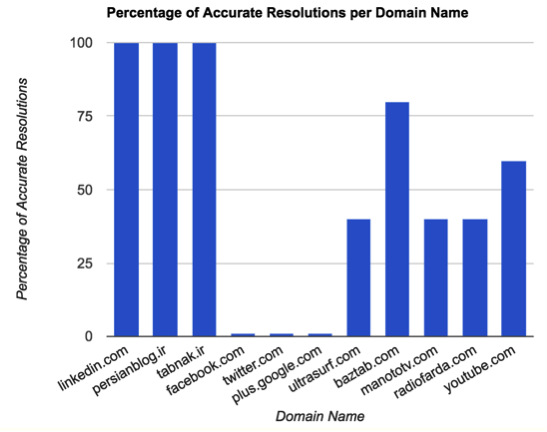
\includegraphics[
  height=.5\columnwidth,
  width=.9\columnwidth
]{ResolutionRate.png}
  \caption{Resolution rate of some queried domains.}
\end{figure}


\begin{figure}
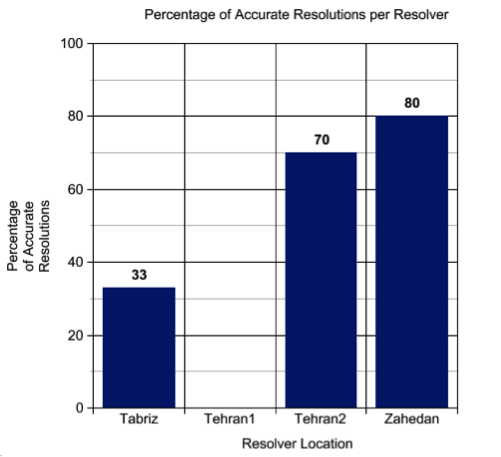
\includegraphics[
  height=.5\columnwidth,
  width=.9\columnwidth
]{PerDNSResolver.png}
  \caption{Percentage accuracy per DNS resolver of domains blocked by at least one resolver}
\end{figure}

